\chapter{Spuštění skriptu}
\subsection*{Virtuální prostředí}
Před spuštěním skriptu je nejprve potřeba vstoupit do virtuálního prostředí, které obsahuje knihovny potřebné ke spuštění skriptu. Pro přístup do virtuálního prostředí je potřeba knihovna \textbf{virtualenv}.

Virtuální prostředí je v~adresáři \textbf{sent10} a lze spustit příkazem:
\begin{center}
    \verb|source sent10/bin/activate|
\end{center}

\subsection*{Vstupní argumenty}
Při spuštění skriptu je nutné zadat několik následujících vstupních argumentů:
\begin{center}
\small
\verb|python3 findReviewArticles.py [reviewProduct] [startDate] [endDate] [parProc]|
\end{center}
\begin{itemize}
    \item \verb|reviewProduct| - Hledaný produkt pro který budou vyhledány recenze.
    \item \verb|startDate| - počáteční datum hledaných recenzí ve formátu \verb|YYYY-MM-DD|
    \item \verb|endDate| - konečné datum hledaných recenzí ve stejném formátu.
    \item \verb|parProc| - počet procesů pro paralelní zpracování.
\end{itemize}

\chapter{Obsah paměťového média}

\begin{itemize}
    \item doc - textová část práce a její zdrojové kódy
    \item models - modely, slovníky a datové sady využité použivané skripty
    \item result - ukázky výsledků práce
    \item Scripts - zdrojové kódy skriptů
    \item sent10 - virtuální prostředí
    \item training - skript a datová sada využitá k~trénování modelu k~určení sentimentu
    \item plakat.pdf - plakát
    \item readme.txt - textový soubor popisující práci, obsahuje návod spuštění skriptů
\end{itemize}


\chapter{Plakát}
\begin{center}
    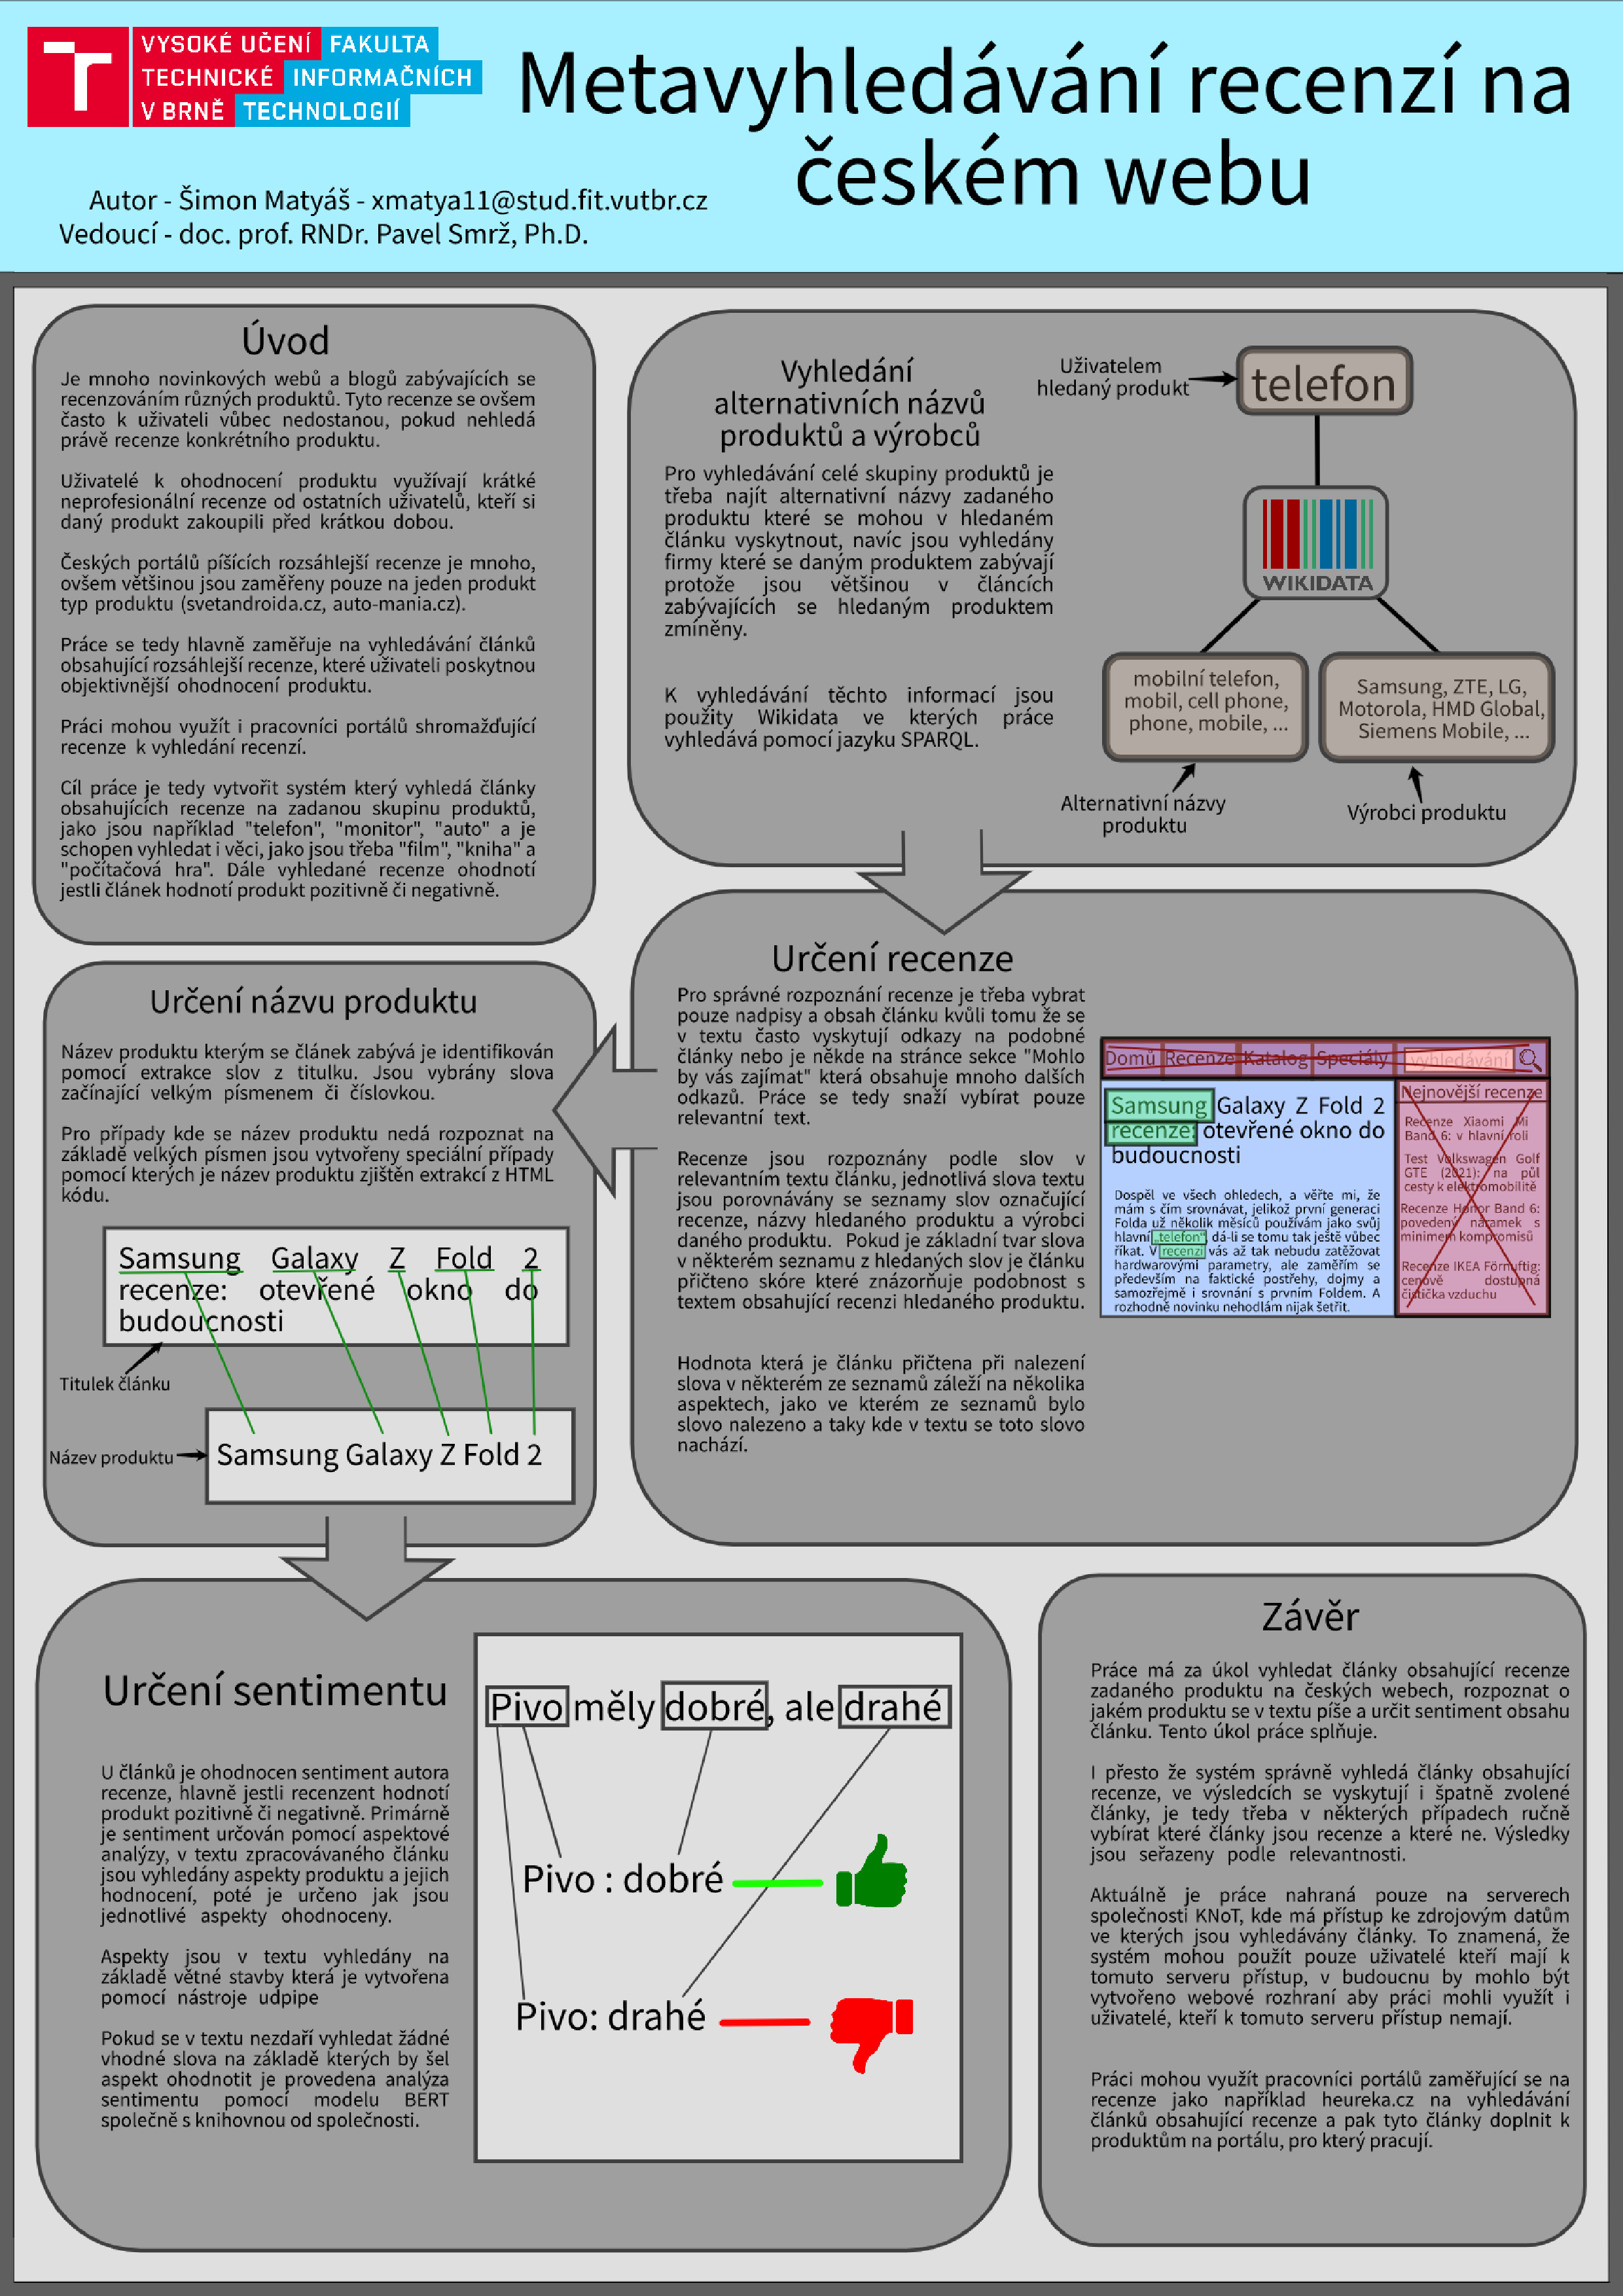
\includegraphics[scale=0.28]{obrazky-figures/plakat.pdf}
\end{center}